\chapter{Statistical Power}

\begin{definition}[Power of a Test]
The probability that a fixed level $\alpha$ significance test will reject $H_0$ when a particular alternative value of the parameter is true is called the \textbf{power} of the test against that alternative.
\end{definition}

The statistical power of a test is its ability to detect an effect if it exists in reality.

It is the probability of correctly rejecting $H_0$ when $H_0$ is false in reality.

\begin{equation*}
\text{Power} = P(\text{reject } H_0 \mid H_0 \text{ false})
\end{equation*}

\begin{equation*}
0 < \text{power} < 1
\end{equation*}

Power close to 1 (high power):\\
\quad Test is good at detecting effects.\\

Power close to 0 (low power):\\
\quad Test is not reliable (i.e., we expect the test will not reject $H_0$ when $H_0$ is false).

\vspace{1em}
Power is affected by:

\begin{itemize}
 \item \textbf{The effect} \\ (\textcolor{blue}{larger differences between reality and the null are easier to detect})

  \item \textbf{Sample size} \\ (\textcolor{blue}{larger samples increase power})

  \item \textbf{Significance level} ($\alpha$) \\ (\textcolor{blue}{as $\alpha$ increases, easier to reject $H_0$})

  \item \textbf{Variability in data} \\ (\textcolor{blue}{lower variability, higher power})
\end{itemize}
\section*{Type I and II Errors}

It is possible to make an incorrect conclusion on a hypothesis test. \\

\textbf{Type I:} Incorrectly reject $H_0$ when $H_0$ is true in reality. \\
\textbf{Type II:} Incorrectly fail to reject $H_0$ when $H_0$ is false in reality. \\


\noindent \textbf{Reality vs Conclusion Table:}
\vspace{1em}
\begin{center}
\small
\renewcommand{\arraystretch}{1.8}
\setlength{\tabcolsep}{1.5em}

\text{Reality}

\vspace{0.5em}

\begin{tabular}{c c}
\hspace*{2em}\rotatebox[origin=c]{90}{\textbf{Conclusion}} &
\begin{tabular}{|l|c|c|}
\hline
& $H_0$ True & $H_0$ False \\
\hline
\textbf{Reject $H_0$} & \textcolor{red}{Type I ($\alpha$)} & \textcolor{green!50!black}{No error \checkmark} \\
\hline
\textbf{Fail to reject $H_0$} & \textcolor{green!50!black}{No error \checkmark} & \textcolor{red}{Type II ($\beta$)} \\
\hline
\end{tabular}
\end{tabular}
\end{center}



\vspace{1em}
\textbf{\textit{Note:}} Type I errors are generally considered worse.

\vspace{0.5em}
\noindent Let $\beta$ be the probability of a Type II error. Then:

\[
\text{Power} = 1 - \beta = 1 - P(\text{Type II})
\]
\begin{example}[Sweetening Colas: Power]
The cola maker determines that a sweetness loss is too large to accept if the mean response for all tasters is $\mu = 1.1$. Will a 5\% significance test detect this?

\textbf{Hypotheses:}
\[
\begin{aligned}
H_0\!:&\ \mu = 0 \\
H_A\!:&\ \mu > 0
\end{aligned}
\]

Assume:
\[
n = 10, \quad \sigma = 1, \quad \alpha = 0.05
\]

\textbf{Step 1: Determine the rejection region.}

Since the test is one-sided with $\alpha = 0.05$, we find:
\[
z_{\text{crit}} = 1.645 \quad \text{(from Z-table)}
\]

We reject $H_0$ if:
\[
Z^* > 1.645
\]

\begin{center}
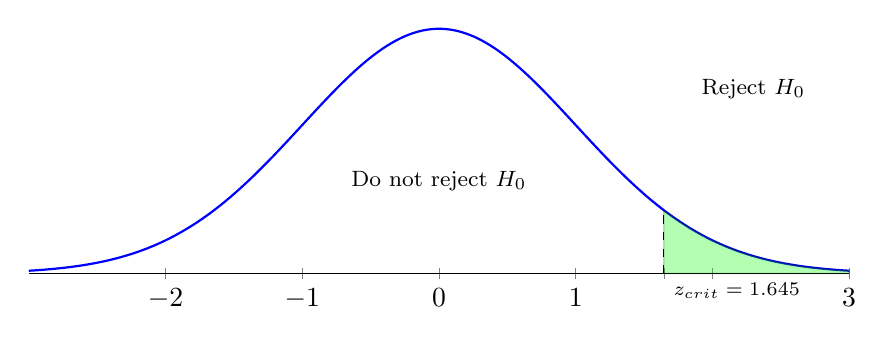
\begin{tikzpicture}
\begin{axis}[
  domain=-3:3,
  samples=200,
  xlabel={},
  ylabel={},
  ymin=0,
  xtick={-2,-1,0,1,1.645,2,3},
  xticklabels={$-2$,$-1$,$0$,$1$,,,$3$},
  ytick=\empty,
  width=12cm,
  height=5cm,
  clip=false,
  axis x line=bottom,
  axis y line=none,
  axis line style={-}, % ensures it's a regular solid line
]

% Standard normal curve
\addplot[blue, thick, no markers, domain=-3:3, samples=200] {exp(-x^2/2)/sqrt(2*pi)};

% Rejection region
\addplot[domain=1.645:3, fill=green, opacity=0.3] {exp(-x^2/2)/sqrt(2*pi)} \closedcycle;

% Critical line
\draw[dashed] (axis cs:1.645,0) -- (axis cs:1.645,{exp(-1.645^2/2)/sqrt(2*pi)});
\node[below right] at (axis cs:1.645,0) {\scriptsize $z_{\text{crit}} = 1.645$};

% Add regions
\node at (axis cs:0, 0.15) {\footnotesize Do not reject $H_0$};
\node at (axis cs:2.3, 0.3) {\footnotesize Reject $H_0$};


\end{axis}
\end{tikzpicture}
\vspace{0.5em}
\captionof{figure}{Rejection region for $Z$ with $\alpha = 0.05$}
\end{center}


\textbf{Step 2: Find the equivalent critical value of } $\bar{x}$.

Since $\sigma$ is known,
\[
Z = \frac{\bar{x} - \mu_0}{\sigma/\sqrt{n}} \quad \Rightarrow \quad
1.645 = \frac{\bar{x}_{\text{crit}} - 0}{1/\sqrt{10}} \Rightarrow \bar{x}_{\text{crit}} \approx 0.520
\]

So we reject $H_0$ if $\bar{x} > 0.520$.

\textbf{Step 3: Calculate the power when $\mu = 1.1$ is true.}

\[
P\left(Z > \frac{0.520 - 1.1}{1/\sqrt{10}}\right)
\approx P(Z > -1.83) = 1 - 0.0336 = 0.9664
\]


\textbf{Interpretation:} There is a 96.6\% chance the test correctly detects $\mu = 1.1$.

\vspace{1em}

\begin{center}
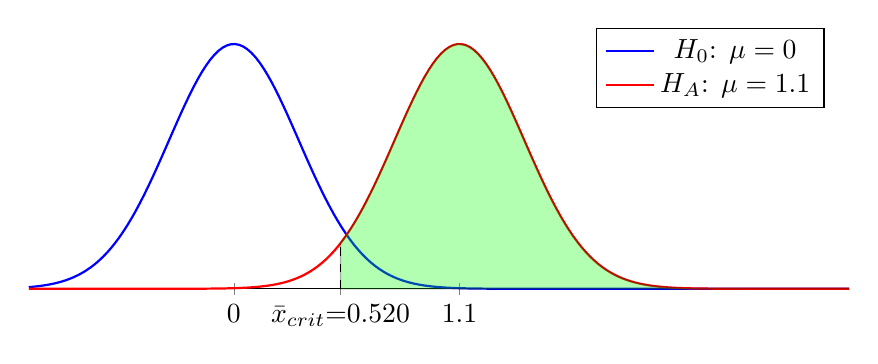
\begin{tikzpicture}
\begin{axis}[
  domain=-1:3,
  samples=200,
  xlabel={},
  ylabel={},
  ymin=0,
  xtick={0,0.52,1.1},
  xticklabels={$0$, $\bar{x}_{\text{crit}}{=}0.520$, $1.1$},
  ytick=\empty,
  width=12cm,
  height=5cm,
  clip=false,
  axis x line=bottom,
  axis y line=none,
  axis line style={-}, % ensures it's a regular solid line
  legend style={at={(0.97,0.97)}, anchor=north east},
]

% H0 distribution (mean = 0)
\addplot[blue, thick] {exp(-(x)^2/(2 * (1/sqrt(10))^2)) / (sqrt(2*pi) * (1/sqrt(10)))};
\addlegendentry{$H_0$: $\mu = 0$}

% HA distribution (mean = 1.1)
\addplot[red, thick] {exp(-(x - 1.1)^2/(2 * (1/sqrt(10))^2)) / (sqrt(2*pi) * (1/sqrt(10)))};
\addlegendentry{$H_A$: $\mu = 1.1$}

% Shade rejection region under H_A
\addplot[domain=0.52:3, fill=green, opacity=0.3] 
  {exp(-(x - 1.1)^2/(2 * (1/sqrt(10))^2)) / (sqrt(2*pi) * (1/sqrt(10)))} 
  \closedcycle;

% Dashed line for x_crit
\draw[dashed] (axis cs:0.52,0) -- (axis cs:0.52, {exp(-(0.52 - 1.1)^2/(2 * (1/sqrt(10))^2)) / (sqrt(2*pi) * (1/sqrt(10)))});
\end{axis}
\end{tikzpicture}
\vspace{0.5em}
\captionof{figure}{Power curve showing shaded rejection area under $H_A$}
\end{center}

\end{example}


